\documentclass[letterpaper,12pt]{article}

\title{Título del documento}
\author{Rodrigo Segura Moreno}
\date {\today }

%% Matemáticas
\usepackage{amsmath}
\usepackage{amssymb}

\usepackage{upgreek} % Greek alphabet

\usepackage{hyperref} % URL
\usepackage{xcolor} % Colores

\usepackage{changepage} % Margins

\usepackage[letterpaper, margin=1 in]{geometry}
\usepackage{graphicx}

\usepackage{gensymb} % Generic symbols for both text and math mode.

\usepackage{systeme}

\begin{document}
	
	\thispagestyle{empty}
	
	\begin{figure}
		\minipage{0.76\textwidth}
			
\includegraphics[ width = 1.65in,height=1.65in ]{FC.jpg}
		\endminipage
		\minipage{0.32\textwidth}
			
\includegraphics[ width = 1.25in,height=1.25in ]{UNAM.png}
		\endminipage
	\end{figure}

	\vspace{0.5cm}
	
	\begin{center}
		\textbf{\large Universidad Nacional Autónoma de México \\}
		\textbf{\large Facultad de Ciencias} \\
		
		\vspace{0.7cm}
		
		{\large  \textbf{Computación} \\}
		\textbf{Grupo:} 8093\\
		Dr. Sergio Antonio Alcalá Corona\\
		Fis. Sergio Ángel Sánchez Chávez
		
		\vspace{0.5cm}
		
		{\large Tarea Programa en LaTeX \\}
		11 de diciembre de 2020
		
		\vspace{0.7cm}
		
		Rodrigo Segura Moreno \\
		
	\end{center}

	\vspace{5pt}
	\hrule
	\vspace{3em}

	El script a desarrollar en Python deberá ser capaz de calcular el volumen de los siguientes sólidos platónicos regulares
	\begin{itemize}
		\item Tetraedro
		\item Octaedro
		\item Icosaedro
	\end{itemize}

	Los sólidos platónicos regulares tienen la peculiaridad que todas sus aristas son de igual longitud.
	
	\minipage{0.32\textwidth}
		\begin{center}
			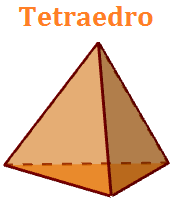
\includegraphics[scale=0.5]{tetraedro.png}
		\end{center}
	\endminipage
	\minipage{0.32\textwidth}
		\begin{center}
			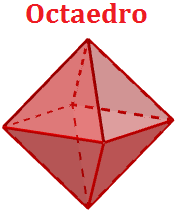
\includegraphics[scale=0.5]{octaedro.png}
		\end{center}		
	\endminipage
	\minipage{0.32\textwidth}
		\begin{center}
			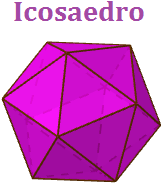
\includegraphics[scale=0.5]{icosaedro.png}
		\end{center}
	\endminipage
	
\end{document}